\chapter{Results}
\label{cha:results}

This chapter is divided into results for selecting models and the evaluation of the unseen validation data using those models. 


\section{Model Selection}
\label{sec:model-selection-result}

With the balanced training and test data different models were trained and the results are shown in tables. 
The best values are marked in bold along with the true numbers for the confusion matrix. 


\begin{table}[H]
    \centering
    \caption{Model result on train data.}
    \label{tab:train-table}
    \begin{tabular}{@{}llllll@{}}
    \toprule
    Model                         & TP             & FP            & FN            & TN             & Accuracy      \\ \midrule
    Dummy Classifier (stratified) & 24015          & 24172         & 24179         & 24221          & 0.50          \\
    Multinomial Naive Bayes       & 41980          & 6207          & 5356          & 43044          & 0.88          \\
    Linear SVM (SGD)              & 40443          & 7744          & 3350          & 45050          & 0.89          \\
    Logistic Regression           & \textbf{42155} & \textbf{6032} & 3049          & 45351          & \textbf{0.91} \\
    KNN                           & 34689          & 13498         & \textbf{2900} & \textbf{45500} & 0.83          \\
    Random Subspaces (SVM)        & 38322          & 9865          & 6028          & 42372          & 0.84          \\ \midrule
    \textbf{True Classification}  & \textbf{48187} & \textbf{0}    & \textbf{0}    & \textbf{48400} & \textbf{}    
    \end{tabular}
\end{table}


Result from training data is listed in table \ref{tab:train-table}. 
For training Logistic Regression (LR) had best precision, as seen with high number of TP and low number of FP. 
KNN instead has the best negative predictive value, low number of FN and high number of TN. 
The dummy classifier performs worst with 50\% accuracy which is however the perfect score for a balance dataset with stratified dummy classifier. 
Linear SVM and Multinomial Naive Bayes (MNB) have similar performance where MNB has slightly better values for positive predictions and SVM for negative predictions. 
Best accuracy is gotten from Logistic Regression with 91\% accuracy. 
The more complex Random Subspace model with very basic parametrization still gets 84\% accuracy, about same as KNN and slightly less than the other models.


\begin{table}[H]
    \centering
    \caption{Model result on test data.}
    \label{tab:test-table}
    \begin{tabular}{@{}llllll@{}}
    \toprule
    Model                         & TP             & FP            & FN            & TN             & Accuracy      \\ \midrule
    Dummy Classifier (stratified) & 10480          & 10324         & 10276         & 10315          & 0.50          \\
    Multinomial Naive Bayes       & \textbf{18042} & \textbf{2762} & 2841          & 17750          & \textbf{0.86} \\
    Linear SVM (SGD)              & 16851          & 3953          & 1794          & 18797          & \textbf{0.86} \\
    Logistic Regression           & 17084          & 3720          & 2015          & 18576          & \textbf{0.86} \\
    KNN                           & 13461          & 7343          & \textbf{1709} & \textbf{18882} & 0.78          \\
    Random Subspaces (SVM)        & 16446          & 4358          & 3005          & 17586          & 0.82          \\ \midrule
    \textbf{True Classification}  & \textbf{20804} & \textbf{0}    & \textbf{0}    & \textbf{20591} & \textbf{}    
    \end{tabular}
\end{table}


Using the test data, table \ref{tab:test-table} there is quite a big shift in results, suggesting the different generalizations between the models. 
The dummy classifier is the same as on the training data, as expected with balanced dataset. 
Now MNB has the best precision and KNN the best negative predictive value. 
KNN has the lowest accuracy at 78\% of the real models, despite having the best negative predictive value. 
Overall the accuracy is just a bit lower than the training data with MNB, SVM and LR all on 86\% and will be used for the Majority Voting. 


\begin{table}[H]
    \centering
    \caption{Majority Voting on test data.}
    \label{tab:voting-table}
    \begin{tabular}{@{}llllll@{}}
    \toprule
    Model                  & TP    & FP   & FN   & TN    & Accuracy \\ \midrule
    Majority Voting     & 17210 & 3594 & 1891 & 18700 & 0.87     \\ \bottomrule
    \end{tabular}
\end{table}


In table \ref{tab:voting-table} is the result from Majority Voting, which was only performed on the test data. 
Compared to the results in table \ref{tab:test-table} the confusion matrix is a combination of the three models used, while accuracy is slightly improved to 87\%. 
This makes Majority Voting using Multinomial Naive Bayes, Linear SVM and Logistic Regression the most accurate of the methods presented. 


\section{Evaluation}
\label{sec:evaluation-result}

For the evaluation all training and test data is used for training the final models Multinomial Naive Bayes, Linear SVM, Logistic Regression and Majority Voting. 

\begin{table}[H]
    \centering
    \caption{Model result on validation data.}
    \label{tab:validation-table}
    \begin{tabular}{@{}llllll@{}}
    \toprule
    Model                        & TP             & FP            & FN            & TN             & Accuracy      \\ \midrule
    Multinomial Naive Bayes      & \textbf{8839}  & \textbf{1828} & 2945          & 10721          & 0.80          \\
    Linear SVM (SGD)             & 8137           & 2530          & \textbf{1746} & \textbf{11920} & 0.82          \\
    Logistic Regression          & 8342           & 2325          & 2092          & 11574          & 0.82          \\
    Majority Voting              & 8420           & 2247          & 1914          & 11752          & \textbf{0.83} \\ \midrule
    \textbf{True Classification} & \textbf{10667} & \textbf{0}    & \textbf{0}    & \textbf{13666} &              
    \end{tabular}
\end{table}

From table \ref{tab:validation-table} it is shown that MNB has best precision while SVM has best negative predictive value. 
The accuracies for the models are about the same with the combination through Majority Voting being the highest at 83\%.


Comparing the predicted, figure \ref{fig:plot-comp1}, with the true labels, figure \ref{fig:plot-comp2}, by plotting positive and negative reviews. 
There is only a slight difference seen in the comparison due to the scaling. 
Looking at the axis there is a small difference in maximum negative reviews and a small difference in positive reviews just behind the peak. 

\begin{figure}[H]
    \centering
    \begin{subfigure}[b]{0.9\textwidth}
        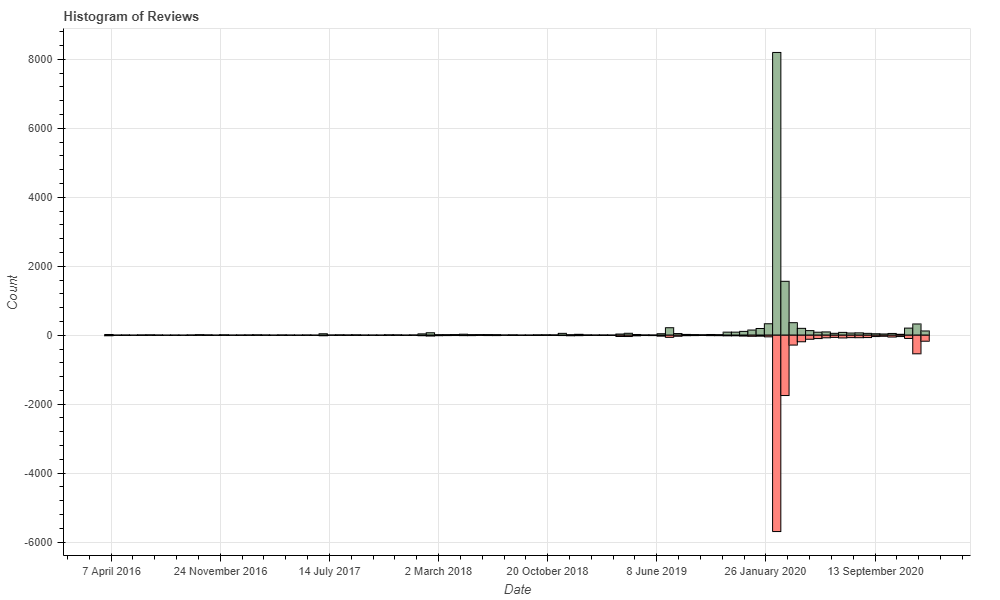
\includegraphics[width=1\textwidth]{../plots/validation_plot.png}
       \caption{}
       \label{fig:plot-comp1} 
    \end{subfigure}
    
    \begin{subfigure}[b]{0.9\textwidth}
        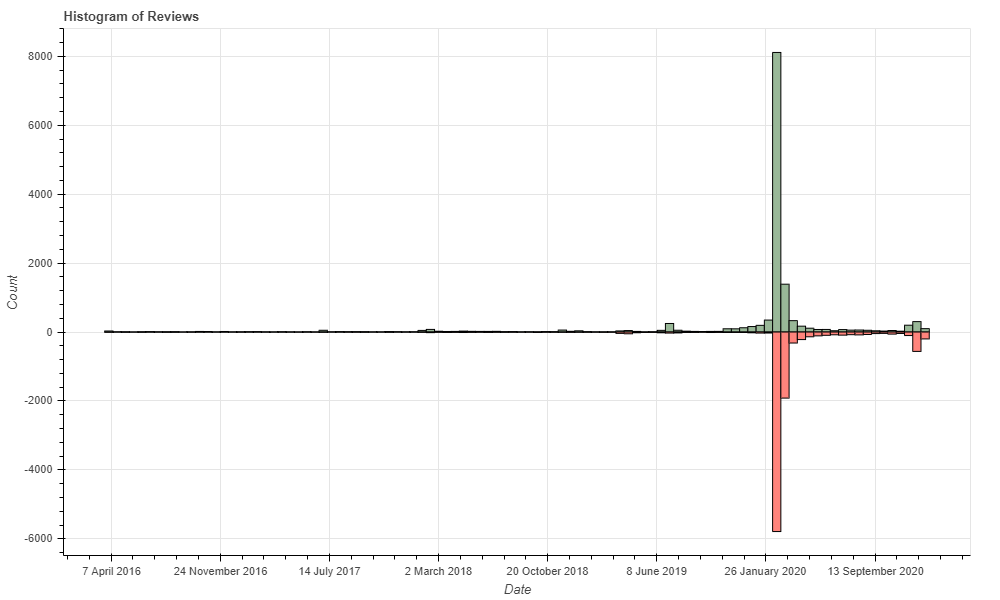
\includegraphics[width=1\textwidth]{../plots/true_plot.png}
       \caption{}
       \label{fig:plot-comp2}
    \end{subfigure}
    
    \caption[Plot of Reviews]{(a) The predicted sentiment from the reviews. (b) The true labels of the reviews.}
\end{figure}


If the plots are scaled using log base 10 a larger difference can be observed between the predicted, figure \ref{fig:plot-comp1-log}, and true figure \ref{fig:plot-comp1-log}. 


\begin{figure}[H]
    \centering
    \begin{subfigure}[b]{0.9\textwidth}
        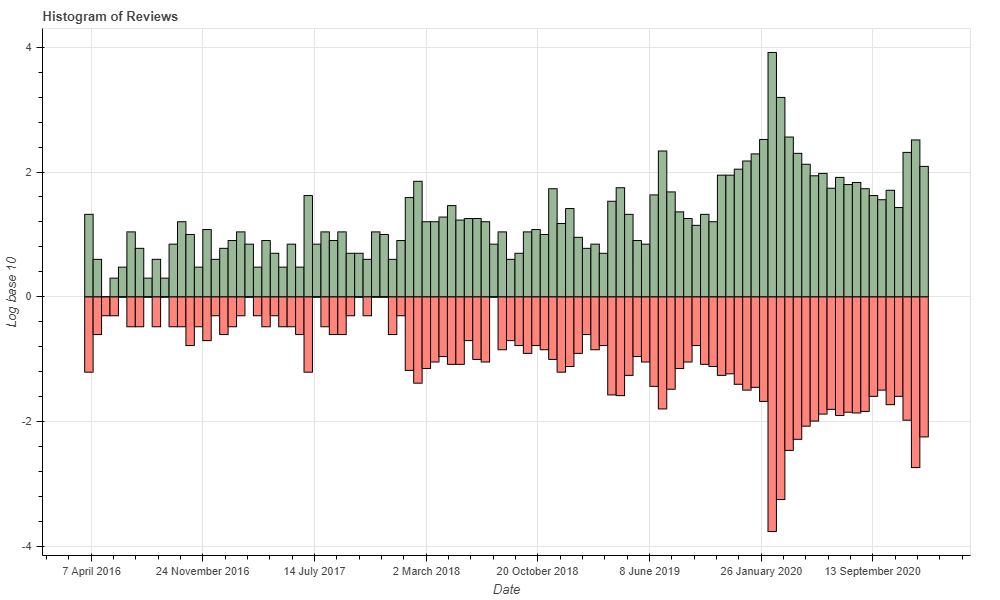
\includegraphics[width=1\textwidth]{../plots/validation_plot_log.png}
       \caption{}
       \label{fig:plot-comp1-log} 
    \end{subfigure}
    
    \begin{subfigure}[b]{0.9\textwidth}
        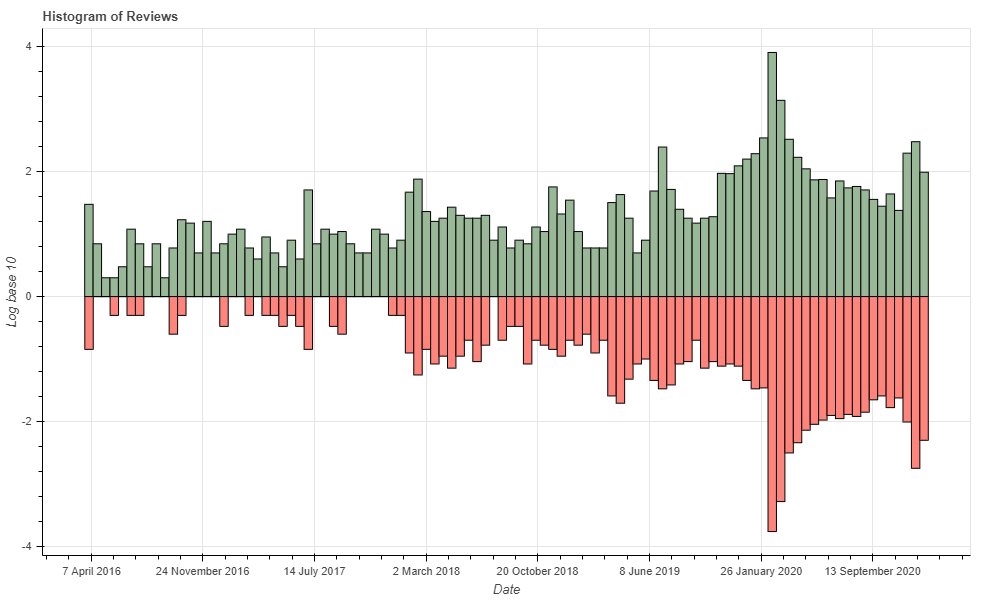
\includegraphics[width=1\textwidth]{../plots/true_plot_log.png}
       \caption{}
       \label{fig:plot-comp2-log}
    \end{subfigure}
    
    \caption[Plot of Scaled Reviews]{(a) The predicted sentiment from the reviews in log base 10. (b) The true labels of the reviews in log base 10.}
\end{figure}


Here a few more differences are found due to the scaling, mostly in the left part of the plots with few reviews since this is sensitive to scaling. 


\begin{figure}[h]
    \caption{Plot showing the tool tip when hovering a bin.}
    \label{fig:hover-tool}
    \centering
    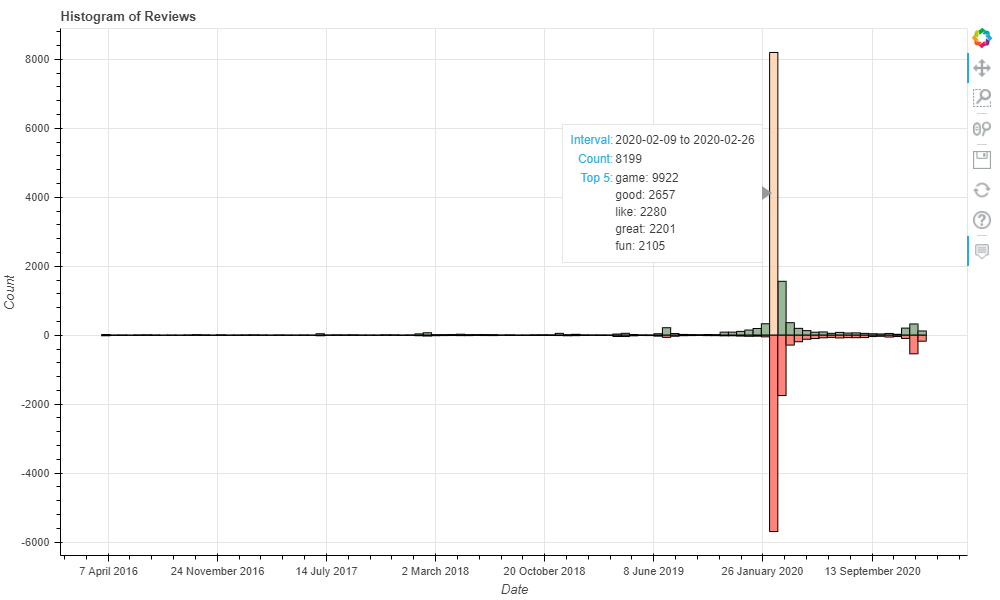
\includegraphics[width=0.9\textwidth]{../plots/demo.png}
\end{figure}

Using the tool tips in the hover tool, as demonstrated in figure \ref{fig:hover-tool}, keywords can be extracted from the different bins. 
This could be useful for a further analysis and see if the top words for positive and negative reviews respectively are changing over time. 
An example of words found is listed in table \ref{tab:words}.


\begin{table}[H]
    \centering
    \caption{Example of most common positive and negative words.}
    \label{tab:words}
    \begin{tabular}{@{}ll@{}}
    \toprule
    Positive & Negative \\ \midrule
    game     & game     \\
    good     & just     \\
    like     & play     \\
    great    & bugs     \\
    fun      & like     \\
    great    & time     \\ \bottomrule
    \end{tabular}
\end{table}